%% Based on a TeXnicCenter-Template by Gyorgy SZEIDL.
%%%%%%%%%%%%%%%%%%%%%%%%%%%%%%%%%%%%%%%%%%%%%%%%%%%%%%%%%%%%%

%------------------------------------------------------------
%
\documentclass{article}%
%Options -- Point size:  10pt (default), 11pt, 12pt
%        -- Paper size:  letterpaper (default), a4paper, a5paper, b5paper
%                        legalpaper, executivepaper
%        -- Orientation  (portrait is the default)
%                        landscape
%        -- Print size:  oneside (default), twoside
%        -- Quality      final(default), draft
%        -- Title page   notitlepage, titlepage(default)
%        -- Columns      onecolumn(default), twocolumn
%        -- Equation numbering (equation numbers on the right is the default)
%                        leqno
%        -- Displayed equations (centered is the default)
%                        fleqn (equations start at the same distance from the right side)
%        -- Open bibliography style (closed is the default)
%                        openbib
% For instance the command
%           \documentclass[a4paper,12pt,leqno]{article}
% ensures that the paper size is a4, the fonts are typeset at the size 12p
% and the equation numbers are on the left side
%
\usepackage{amsmath}%
\usepackage{amsfonts}%
\usepackage{amssymb}%
\usepackage{graphicx}
%-------------------------------------------
\newtheorem{theorem}{Theorem}
\newtheorem{acknowledgement}[theorem]{Acknowledgement}
\newtheorem{algorithm}[theorem]{Algorithm}
\newtheorem{axiom}[theorem]{Axiom}
\newtheorem{case}[theorem]{Case}
\newtheorem{claim}[theorem]{Claim}
\newtheorem{conclusion}[theorem]{Conclusion}
\newtheorem{condition}[theorem]{Condition}
\newtheorem{conjecture}[theorem]{Conjecture}
\newtheorem{corollary}[theorem]{Corollary}
\newtheorem{criterion}[theorem]{Criterion}
\newtheorem{definition}[theorem]{Definition}
\newtheorem{example}[theorem]{Example}
\newtheorem{exercise}[theorem]{Exercise}
\newtheorem{lemma}[theorem]{Lemma}
\newtheorem{notation}[theorem]{Notation}
\newtheorem{problem}[theorem]{Problem}
\newtheorem{proposition}[theorem]{Proposition}
\newtheorem{remark}[theorem]{Remark}
\newtheorem{solution}[theorem]{Solution}
\newtheorem{summary}[theorem]{Summary}
\newenvironment{proof}[1][Proof]{\textbf{#1.} }{\ \rule{0.5em}{0.5em}}

\begin{document}

\title{Exploring and Modeling with the IMDB Movie Dataset}
\author{Sayma Akther, Md. Kauser Ahmmed, 
\\Soujanya Chatterjee, Anjana Tiha, Md. Azim Ullah
\\University of Memphis}
\date{December 06, 2016}
\maketitle

\section{Introduction}

Movies can be of different stories, genre, from different countries, having different actors (both male and female), directors and others. There are several sources in the internet today that stream our favorite movies on demand, that is whenever you want and as often you want, Netflix for example. We all love to watch movies. It is one of the best entertainer during the leisure hours. \footnote{Please find all the figures in the Appendix section below}

\subsection{Goal Description}

To predict whether a movie is going to be popular or not or what will the gross income of a particular movie before its release or what will be the IMDB score of a movie or to suggest you a movie quite similar to the one who have just watched. This seems to be exciting, since based on our relied prediction one (from the audience) can go and watch a movie (predicted to be popular and entertaining) or based on the prediction of the gross, the movie makers can change their marketing regime for their next movie given the features. This work will be useful to both the audience and the movie makers. 
In this work, we have done an exploratory analysis and modeling with IMDB movie data set available in an online data science platform, Kaggle. Namely, we have performed visualization, 'value' prediction or regression in the form of predicting the imdb score and gross of a movie, 'class' prediction or classification in the form of predicting the popularity of a movie, and clustering in the form of a basic recommender system.

\subsection{DataSet Description}

We used the IMDB 5000+ movie dataset for our project. The dataset consists of 5043 unique movies and their attributes (28 variables). The collection spans over 100 years and 66 different countries. There are 2399 unique director names and thousands of actors and actresses. The following is the list of 28 variables from the data set,

[movietitle, color, numcriticforreviews, moviefacebooklikes, duration, directorname, directorfacebooklikes, actor3name, actor3facebooklikes, actor2name, actor2facebooklikes, actor1name, actor1facebooklikes, gross, genres, numvotedusers, casttotalfacebooklikes, facenumberinposter, plotkeywords, movieimdblink, numuserforreviews, language, country, contentrating, budget titleyear, imdbscore, aspectratio.]

\section{Methods and Experimental Evaluation}
\section{Regression or 'Value' Prediction}
In this work we have developed regression models for predicting, \textit{imdbscore} and \textit{gross} of a movie. First we describe the analysis and methods used for \textit{imdbscore} prediction. \textit{imdbscore} is a score or rating provided to movies by critics by an online databased platform for movies, IMDB\cite{}. This score is able to quantify how popular a movie is. Figure~\ref{fig:imdb_hist} shows a histogram plot for the imdb scores. From the plot we can observe a normal distribution of the score, with a mean = 6.465$\pm$1.056, minimum value of 1.6 for the movie \textit{Justin Beiber: Never say never} and maximum of 9.3 for the movie \textit{Shawshank Redemption}. 
In the data set, we have 28 variables, out of which there are 13 useable numeric features, namely, [directorfacebooklikes, gross, numvotedusers, numcriticforreviews, numuserforreviews, budget, moviefacebooklikes, duration, actor3facebooklikes, actor1facebooklikes, actor2facebooklikes, casttotalfacebooklikes, facenumberinposter], and we have included the profit of a movie, which is calculated by subtracting the budget from the gross. First, we have cleaned the data by dropping those samples having NaN values (using 3756 out of 5043 for modeling) and scaled all the features. For all analysis we have used the numpy, scipy, sklearn, pandas, matplotlib, seaborn and bokeh libraries of python.

\subsection{Prediction of IMDB Score}
\begin{itemize}
\item Initial step: Since this is a regression problem, we just run a simple linear regression using all the numerical features. To be noted for all the linear regression models, we have performed evaluation by running different folds of the training and test samples, that is with trainsize = 0.5, 0.66 and 0.75 and report the mean residue square value and the mean square error. We observe the following results. The mean MSE is 0.013 and mean residual square is $0.296$.
\end{itemize}

\begin{itemize}
\item Second step: Next we analyzed the correlation of these features with the \textit{imdbscore} as shown via the scatter plots in figure~\ref{fig:scatter}. We observe that \textit{numvotedusers} has the highest correlation with \textit{imdbscore}, 0.482 and \textit{facenumberinposter} has a negative correlation of -0.065. We observe that for \textit{directorfacebooklikes} (642 out of 3756 are 0) and \textit{moviefacebooklikes} (1742 out of 3756 are 0) has a lot of missing data, hence, we remove them from our next analysis. Next we again performed a simple linear regression for predicting the \textit{imdbscore}, with the new set of features. We observe the following results. The mean MSE is 0.0126 and mean residual square is 0.323. We observe an improvement from the first step.
\end{itemize}

\begin{itemize}
\item Third step: Next we observe that there are a few text features that might be useful in predicting the \textit{imdbscore}, namely \textit{genre}, \textit{plotkeywords} and \textit{country} since they fit the \textit{imdbscore} better than the other text/categorical features (MSE = 0.016 and residue squared = 0.1). We need to add these to the numerical features. For this, first we obtain the tfidf scores with the tfidf vectorizer and use todense() to convert each feature from sparse to dense matrix. Next we append these feature along with the numerical features to obtain a new feature list to predict the \textit{imdbscore}. We observe the following results. The mean MSE is 0.011 and mean residual square is 0.455. We observe an improvement from the second step.
\end{itemize}

\begin{itemize}
\item Fourth step: Next from the figure~\ref{fig:Correlationoffeatures}, we observe that some of the features are correlated to each other. For example, \textit{numvotedusers} and \textit{numcriticforreviews} have some correlation, similarly \textit{gross} and \textit{numvotedusers} have some correlation, hence in this step we have used LASSO regression, since this method does feature selection by assigning 0 coefficient for those features which are redundant and hence reduces overfitting via first norm regularization. We use aic/bic for evaluating the model. We have found the optimal alpha from a range of alpha values of the LASSO model for which the aic and bic are minimum. We performed cross validation to obtain a mean cross-validation score of 0.471. We observe an improvement from the third step.
\end{itemize}

\begin{itemize}
\item Fifth step: Next we attempted using the Random Forest Resgression to perform the prediction of the \textit{imdbscore}. We performed 5-fold cross validation for the evaluation. We observed the mean cvScore to be 0.511. Another important aspect of random forest is that it provides us with the feature importance list. We note the following top 10 features for \textit{imdbscore} prediction. [numvotedusers, genres, budget, duration, numuserforreviews, gross, numcriticforreviews, directorfacebooklikes, actor3facebooklikes, profit]. 
\end{itemize}

Hence we conclude that random forest regression works best among all the methods used to predict the value of \textit{imdbscore} given the features of a movie. Figure~\ref{fig:Fitplot} shows the fitted vs actual data plot for the three methods used. 

\subsection{Prediction of Gross}
Next we use the movie data set to predict gross of a movie. Both categorical and numerical features of the data have been used to predict gross. It has been treated as regression problem. First, data has been pre-processed. The numerical features have been scaled. We have used 5 numerical features; 3 top actors’ and director’s Facebook likes, budget, and 7 textual/categorical features; 3 top actors’ names, director’s name, country, content rating, language for gross prediction. Textual features have been labeled for each column separately and then they have been transformed to binary form. 

Random Forest Regression and Decision Tree Regression has been used to predict gross. Cross Validation has been applied to evaluate the regression model performance. 5-Fold Cross Validation has used. Cross validation with Mean Absolute Error(MAE) and Mean Squared Error(MSE) has been calculated. Figure~\ref{fig:RFR} shows the plot for actual v predicted gross when using Random Forest Regression. Figure~\ref{fig:DTR} shows the plot for actual v predicted gross when using Decision tree Regression. Table~\ref{tab:gross} displays the results.

\begin{table}[]
\centering
\caption{Gross Prediction}
\label{tab:gross}
\begin{tabular}{|l|l|l|}
\hline
Evaluation Metrics  & Random Forest Regression & Decision Tree Regression \\ \hline
Mean Absolute Error & 0.0398                   & 0.0456                   \\ \hline
Mean Square Error   & 0.0048                   & 0.0065                   \\ \hline
R-Square            & 0.4628                   & 0.3225                   \\ \hline
Explained Var Score & 0.468                    & 0.265                    \\ \hline
\end{tabular}
\end{table}

\section{Classification}

In this section we discuss the two classification problems addressed in this work. First, we build classification models for prediction of high rated or popular (\textit{imdbscore} $>$ 8) and low rated or not so popular movies (\textit{imdbscore} $\leq$ 8). Second, we also build classification models to predict profitable (\textit{profit} $>$ 0) v not profitable movies (\textit{profit} $<$ 0).

To build the model, 11 numerical and 3 text/categorical features were used (same as used in prediction of imdbscore). 

\begin{itemize}
\item Prediction of popular or not so popular movies - First we worked with only the numerical data. Several classification models were employed. We evaluated the models via 5-Fold cross-validation. Table~\ref{tab:Classification_of_High_rated_movie} includes all the results. We observe that decision tree and random forest classifiers work the best. Next we added the text/categorical feature along with the numerical features. Table~\ref{tab:Classification_of_High_rated_movie_NC} includes all the results. Random forest classifier again performs the best. 
\item Prediction of profitable v not profitable movies - First we worked with only the numerical data. Several classification models were employed. We evaluated the models via 5-Fold cross-validation. Table~\ref{tab:Classification_of_profit_movie} includes all the results. We observe that decision tree and logistic regression classifiers work the best. Next we added the text/categorical feature along with the numerical features. Table~\ref{tab:Classification_of_profit_movie_NC} includes all the results. Support Vector classifier again performs the best. 
\item Observation - In both the cases we observe that classification performance drops on addition of text/categorical features. 
\end{itemize}

\begin{table}[tb]
\caption{Classification of High rated movie(Numerical features)}
\label{tab:Classification_of_High_rated_movie}
\begin{center}
\footnotesize
\begin{tabular}{|c|c|c|c|} \hline
%\toprule
\textbf{Model Name}& \textbf{Precision}& \textbf{Recall} & \textbf{F1-score }   \\ \hline \hline
Decision Tree method &	1.00	& 1.00 &	1.00\\ \hline
Extra Trees method &	0.98	& 0.98 &	0.98\\ \hline
Random Forest method &	1.00	&1.00&	1.00\\ \hline
SVC method &	0.95	& 0.95 &	0.92\\ \hline
Logit method&	0.93&	0.95&	0.93\\ \hline
GaussianNaiveBayes method&	0.92	&0.91	&0.92\\ \hline

%\bottomrule
\end{tabular}
\end{center}
\end{table}



\begin{table}[tb]
\caption{Classification of High rated movie(Numerical+ categorical featuress)}
\label{tab:Classification_of_High_rated_movie_NC}
\begin{center}
\footnotesize
\begin{tabular}{|c|c|c|c|} \hline
%\toprule
\textbf{Model Name}& \textbf{Precision}& \textbf{Recall} & \textbf{F1-score }   \\ \hline \hline
Decision Tree method & 0.95	 & 0.95	& 0.95\\ \hline
Extra Trees method & 0.96 &	0.96 &	0.95\\ \hline
Random Forest method & 0.96	& 0.96 &	0.96\\ \hline
SVC method & 0.95 &	0.95	&0.92\\ \hline
Logit method& 0.94	& 0.92 &	0.93\\ \hline
GaussianNaiveBayes method & 0.95 &	0.93 &	0.94\\ \hline

%\bottomrule
\end{tabular}
\end{center}
\end{table}


\begin{table}[tb]
\caption{Classification of profitable movie(Numerical features)}
\label{tab:Classification_of_profit_movie}
\begin{center}
\footnotesize
\begin{tabular}{|c|c|c|c|} \hline
%\toprule
\textbf{Model Name}& \textbf{Precision}& \textbf{Recall} & \textbf{F1-score }   \\ \hline \hline
Decision Tree method & 0.97 &	0.97 &	0.97 \\ \hline
Extra Trees method & 0.86	& 0.85 &	0.85\\ \hline
Random Forest method & 0.89 &	0.89	&0.89\\ \hline
SVC method & 0.75 &	0.55	& 0.40\\ \hline
Logit method &  1.00	 &1.00	& 1.00\\ \hline
GaussianNaiveBayes method & 0.54	& 0.55	& 0.46\\ \hline
%\bottomrule
\end{tabular}
\end{center}
\end{table}


\begin{table}[tb]
\caption{Classification of profitable movie(Numerical+ categorical features)}
\label{tab:Classification_of_profit_movie_NC}
\begin{center}
\footnotesize
\begin{tabular}{|c|c|c|c|} \hline
%\toprule
\textbf{Model Name}& \textbf{Precision}& \textbf{Recall} & \textbf{F1-score }   \\ \hline \hline
Decision Tree method & 0.68	& 0.68 &	0.68\\ \hline
Extra Trees method & 0.68 &	0.68	&0.68\\ \hline
Random Forest method & 0.70	 & 0.70 &	0.70\\ \hline
SVC method & 0.75 &	0.55	&0.40\\ \hline
Logit method& 0.70	& 0.70	&0.70\\ \hline
GaussianNaiveBayes method &  0.66	& 0.56 &	0.44\\ \hline

%\bottomrule
\end{tabular}
\end{center}
\end{table}

\section{Clustering}

We used clustering to build a simple movie recommender system. Consider a scenario, where an user would like to find a similar movie to the one he/she has already watched, based on \textit{genre}, \textit{plot key words}, \textit{cast and crews}. This system will be able to suggest top 10 similar movie given the movie watched based on k-means clustering algorithm. 
To build the system, first we produce unique clusters given the features, \textit{genre}, \textit{plot key words}, \textit{cast and crews}, where \textit{cast and crews} includes all the actors and directors. Next, given a movie, we search for other movie in the cluster. Once we have the movie list, then we suggest to the user the top 10 best movies based on their \textit{imdbscore} or \textit{gross}. We also have the autocorrect feature, that is if the movie provided is not in the database, then we suggest the best matches with respect to the provided title. 
We show a screen shot of the system in the figure~\ref{fig:suggestiongross} and figure~\ref{fig:suggestionimdbscore} 

We developed several visualization in the process of performing exploratory analysis of the movie data set. These visualizations help us in understanding the data, extract useful information from the data and then use them for modeling purposes. 

First we build a web based interactive visualizer using the \textit{bokeh} library of python. It includes various options which the user can select from in order to obtain the data visualization according to their query. For example, if one wants to know the relationship between \textit{number of critic reviews} and \textit{imdbscore} for movies starring Brad Pitt then the  user can simply select the required options to get the data visualization displayed on the web page itself. Figure~\ref{fig:webvisualizer} shows a screen shot for this visualization. 

Next we also developed several interesting data exploratory analysis, represented by different plots. 

\begin{itemize}
\item Top 10 rated movies based on IMDB rating - Shawshank Redemption. Figure~\ref{fig:TOP 10 Best Rated Movies} displays the result.
\item Top 10 directors based on critic reviews - Steven Spielberg tops the list Figure~\ref{fig:Directors Ranked on total critic reviews} displays the result.
\item Top 10 actors based on critic reviews in IMDB - Jhonny Depp on the top Figure~\ref{fig:ttanc} displays the result.
\item Top 10 actors based on number of user votes in IMDB - Morgan Freeman on the top Figure~\ref{fig:Top10actorsbasedonnumvotedusers} displays the result.
\item Top 10 actors based on gross in IMDB - Robert Downey Jr. he seems to enjoy a whole lot of money Figure~\ref{fig:Top10actorsbasedongross} display the result.
\item Top 10 countries having most movie budget - USA tops the list. Figure~\ref{fig:crfm} displays the result.
\item Box and Whisker plot to show the distribution of imdb score based on selected year and countries - The year 2007 shows highest median movie ratings. USA produces the maximum films annually however the average imdb scores is far less than those films produced in other countries. Figures~\ref{fig:Box and whisker plotofcountriesbasedonimdbscore} and ~\ref{fig:Box and whisker plotofYearsbasedonimdbscore} display the results.
\item Top 10 profitable movies - Avatar, Jurrasic World and Titanic tops the table. Figure~\ref{fig:TOP10MostProfitableMovies} displays the result.
\item Histogram of face number of posters - Interestingly we find that almost 98\% of posters have less than 5 faces. Figure~\ref{fig:face} displays the result.
\item Top 10 directors raking highest gross - Steven Spielberg tops the list. Figure~\ref{DirectorsRankedontotalgross} displays the result.
\item Top 10 directors raking highest average budget - Joon-ho Bong from South Korea. Interestingly South Korea makes less movies but all of them are of substantial budget. Figure~\ref{DirectorsRankedonAverageBudget.png} displays the result.
\end{itemize}

\begin{figure}
\centering
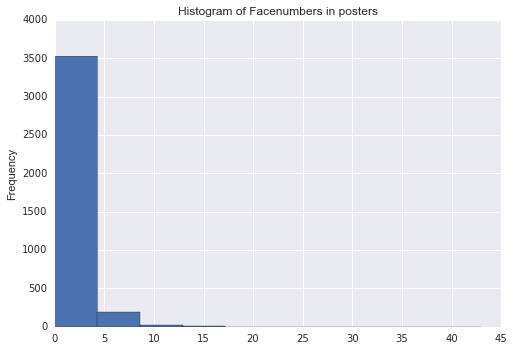
\includegraphics[width=1.0\columnwidth]{Fig/face.png}
\caption{No. of faces on poster}
\label{fig:face}
\end{figure}

\begin{figure}
\centering
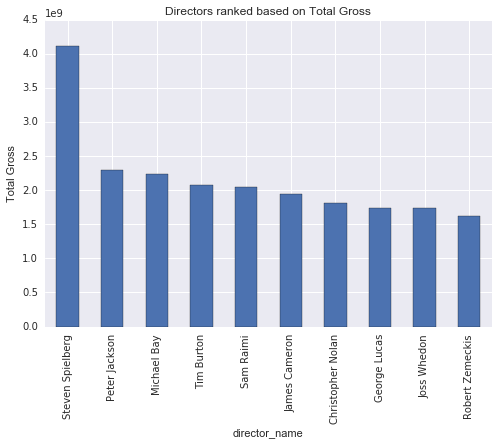
\includegraphics[width=1.0\columnwidth]{Fig/DTGR.png}
\caption{Top 10 Grossing Directors}
\label{fig:DirectorsRankedontotalgross.png}
\end{figure}

\begin{figure}
\centering
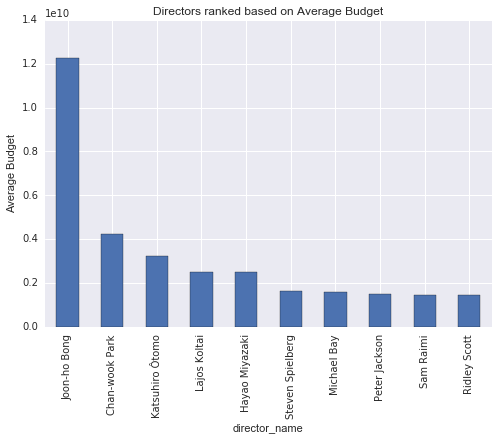
\includegraphics[width=1.0\columnwidth]{Fig/DirectorsRankedonAverageBudget.png}
\caption{Top 10 Directors by average Budget}
\label{fig:DirectorsRankedonAverageBudget}
\end{figure}

\section{Contributions}

\begin{itemize}
\item Sayma Akther - Classification (profitable v non profitable movie and popular v non popular movie) model development, statistical analysis, evaluation and results.
\item Md. Kauser Ahmmed - Clustering and text/categorical feature and statistical analysis for prediction of IMDB Score.
\item Soujanya Chatterjee - Correlation analysis of numerical features, comparative regression model development for prediction of IMDB score, evaluation and results.
\item Anjana Tiha - Data analysis, Visualization for gross prediction using regression models, evaluation and results.
\item Md. Azim Ullah - Interactive web-based visualization development and exploratory statistical data analysis.
\end{itemize}

\section{Apendix}

\begin{figure}
\centering
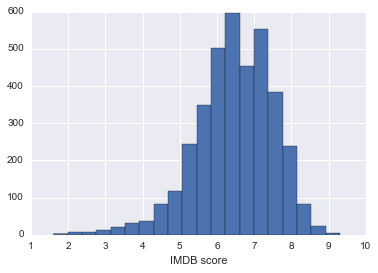
\includegraphics[width=1.0\columnwidth]{Fig/imdbhist.png}
\caption{Histogram plot for imdbscore}
\label{fig:imdbhist}
\end{figure}

\begin{figure}
\centering
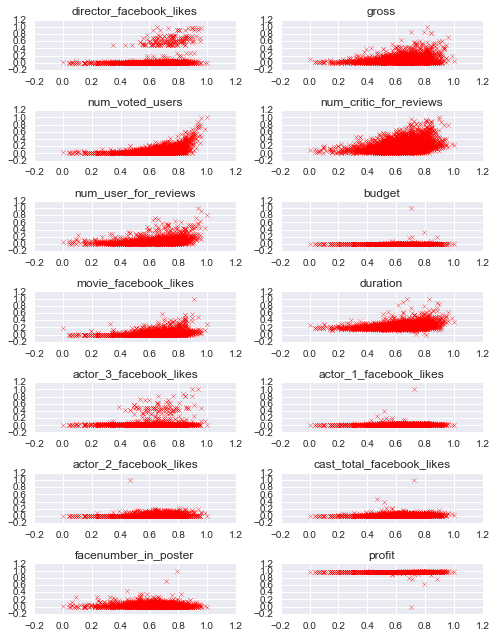
\includegraphics[width=1.0\columnwidth]{Fig/ScatterPlot.png}
\caption{Scatter plot for imdbscore v numerical features}
\label{fig:scatter}
\end{figure}

\begin{figure}
\centering
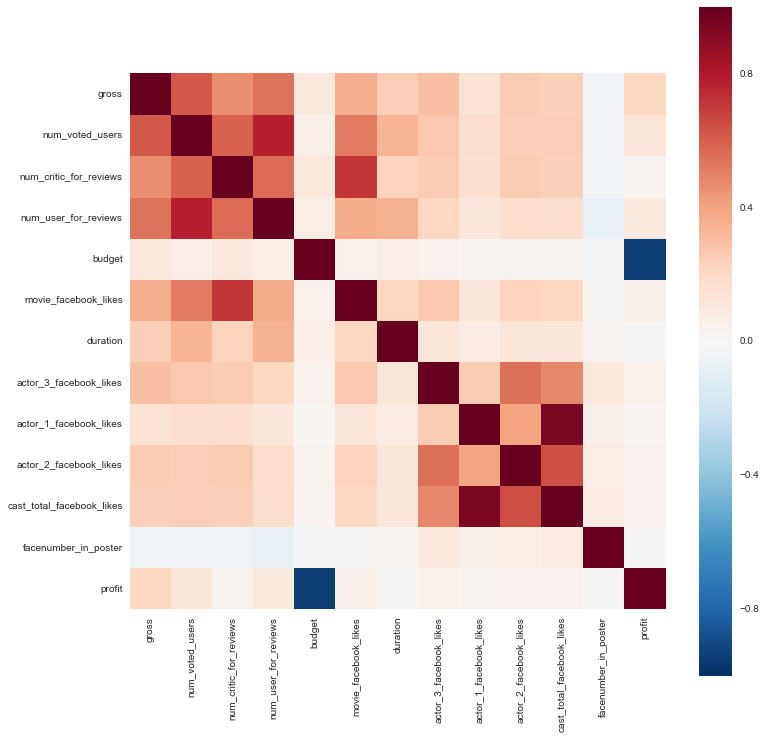
\includegraphics[width=1.0\columnwidth]{Fig/Correlationoffeatures.png}
\caption{Correlation of Numerical features}
\label{fig:Correlationoffeatures}
\end{figure} 

\begin{figure}
\centering
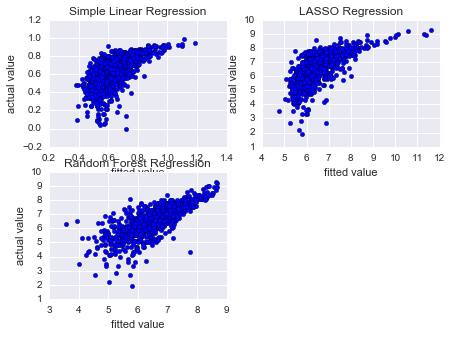
\includegraphics[width=1.0\columnwidth]{Fig/Fitplot.png}
\caption{Fitted vs Actual data plot}
\label{fig:Fitplot}
\end{figure}

\begin{figure}
\centering
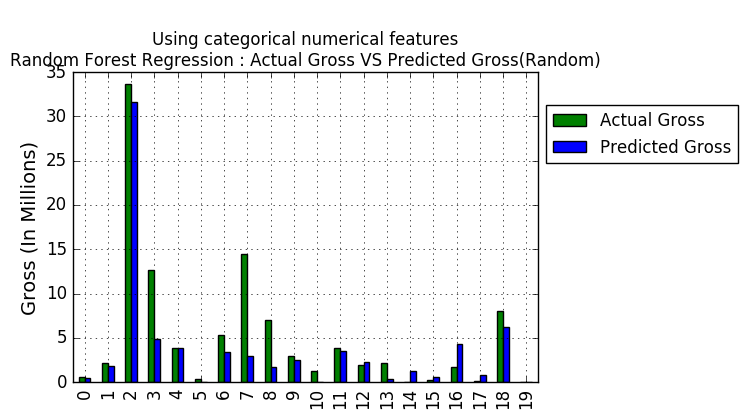
\includegraphics[width=1.0\columnwidth]{Fig/RFR.png}
\caption{Movie Recommendation according to IMDB Score}
\label{fig:RFR}
\end{figure}

\begin{figure}
\centering
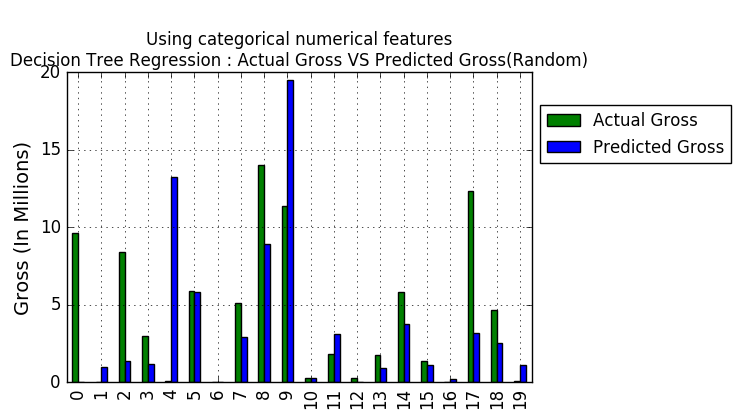
\includegraphics[width=1.0\columnwidth]{Fig/DTR.png}
\caption{Movie Recommendation according to IMDB Score}
\label{fig:DTR}
\end{figure}

\begin{figure}
\centering
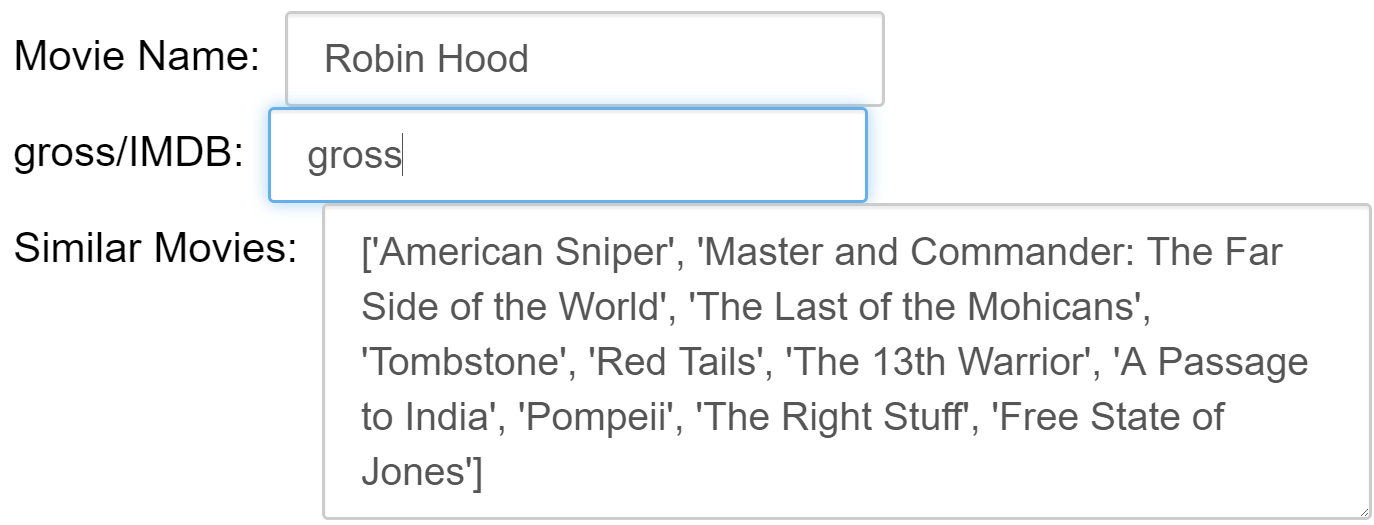
\includegraphics[width=1.0\columnwidth]{Fig/suggestiongross.PNG}
\caption{Movie Recommendation according to gross}
\label{fig:suggestiongross}
\end{figure}

\begin{figure}
\centering
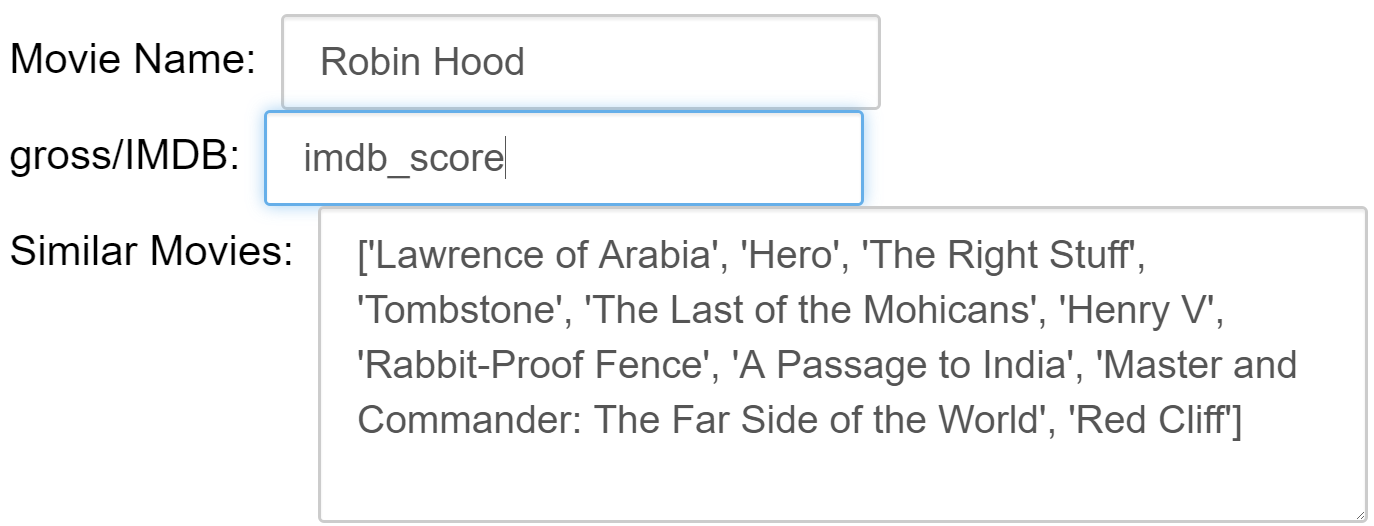
\includegraphics[width=1.0\columnwidth]{Fig/suggestionimdbscore.PNG}
\caption{Movie Recommendation according to IMDB Score}
\label{fig:suggestionimdbscore}
\end{figure}

\begin{figure}
\centering
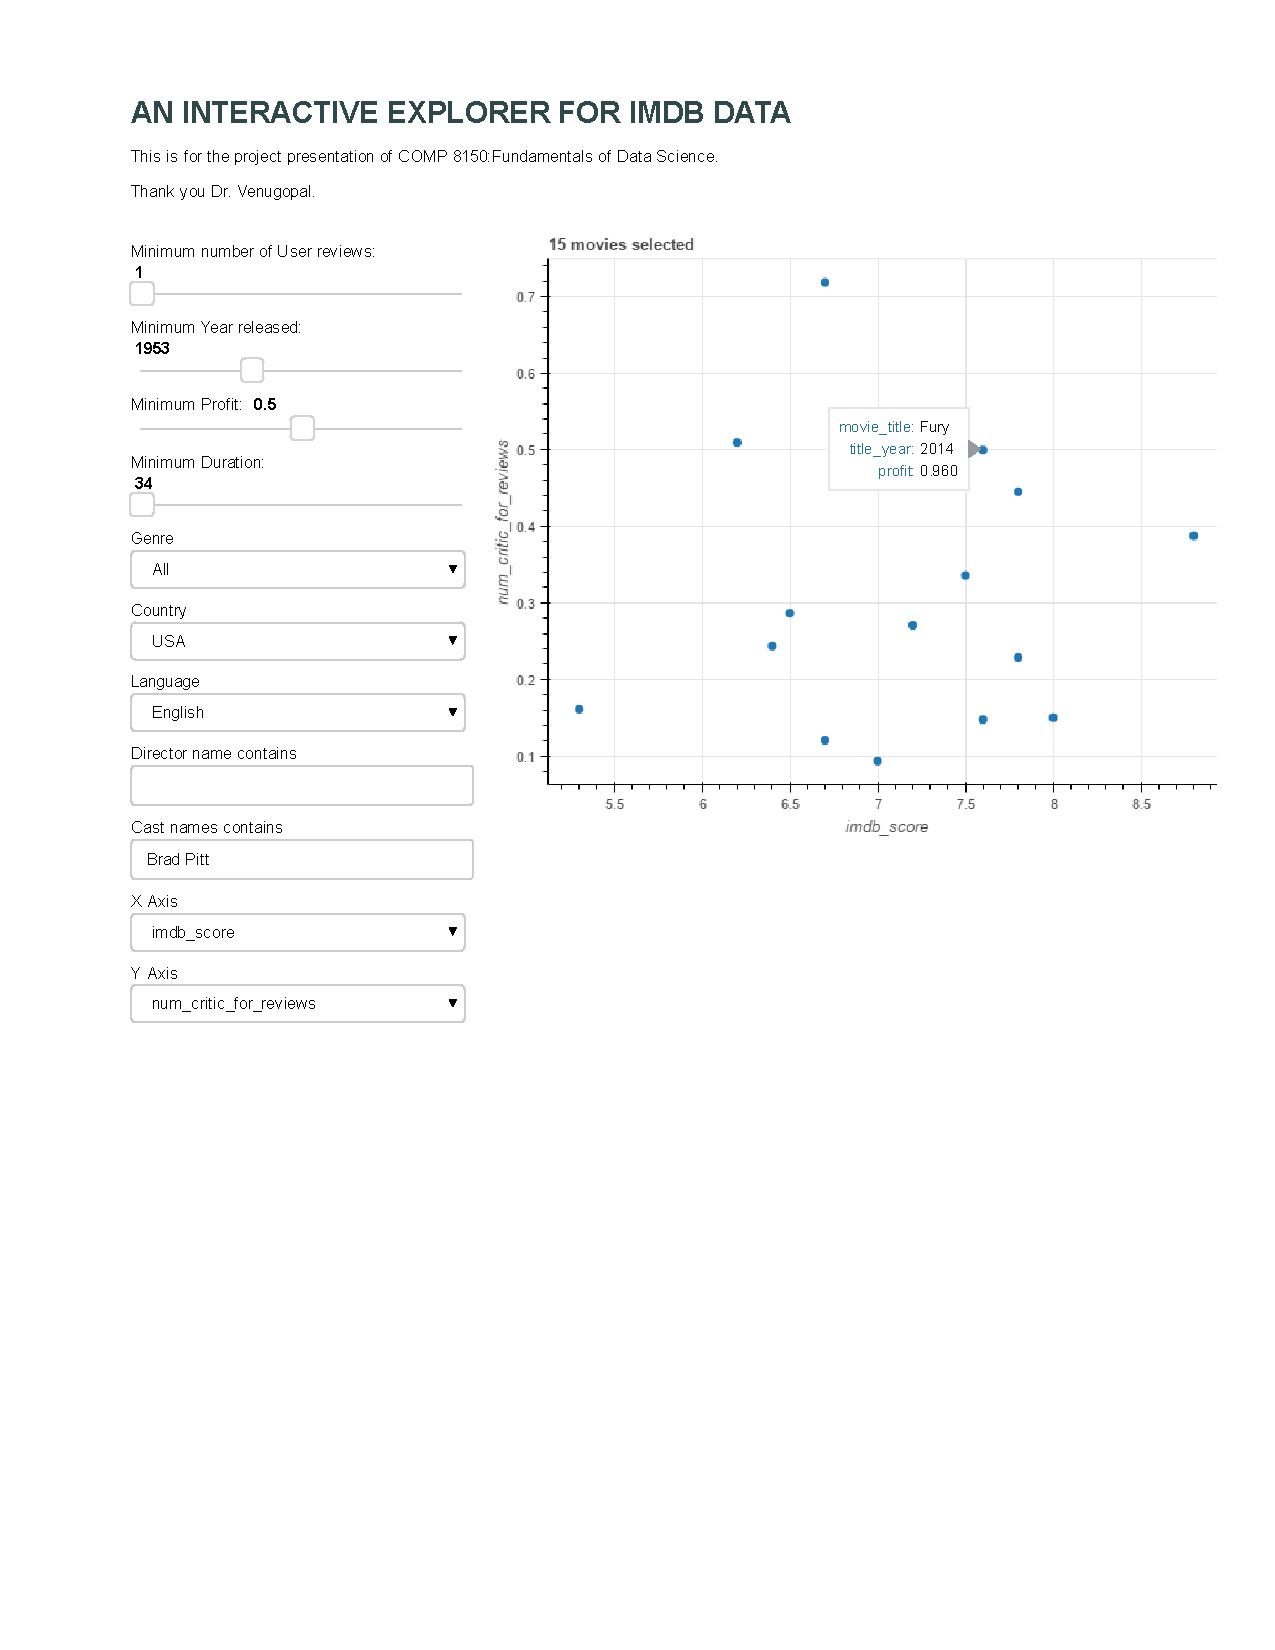
\includegraphics[width=1.0\columnwidth]{Fig/webvisualizer.pdf}
\caption{Interactive web-based Visualizer snapshot}
\label{fig:webvisualizer}
\end{figure}

\begin{figure}
\centering
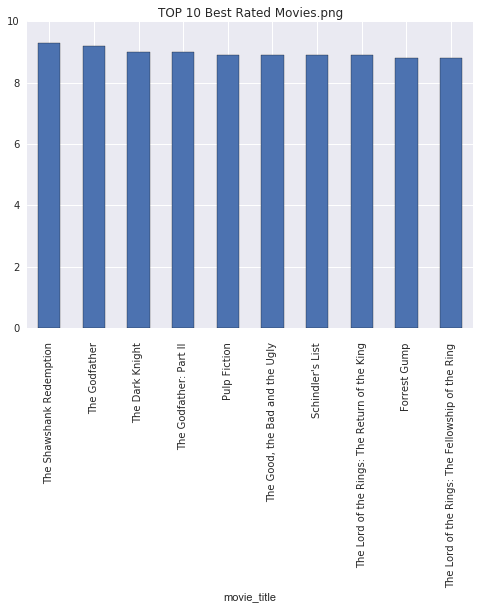
\includegraphics[width=1.0\columnwidth]{Fig/TOP10BestRatedMovies.png}
\caption{Top 10 Best Rated Movies}
\label{fig:TOP 10 Best Rated Movies}
\end{figure}

\begin{figure}
\centering
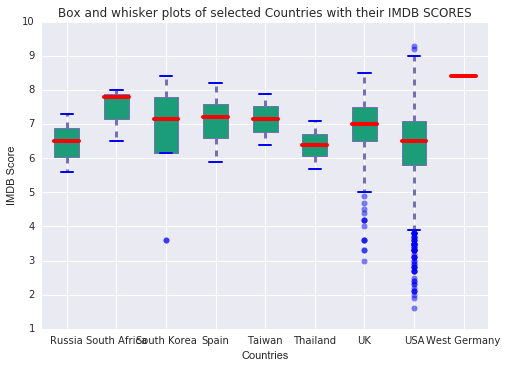
\includegraphics[width=1.0\columnwidth]{Fig/Boxandwhiskerplotofcountriesbasedonimdbscore.png}
\caption{IMDB Score based on Countries}
\label{fig:Box and whisker plotofcountriesbasedonimdbscore}
\end{figure}

\begin{figure}
\centering
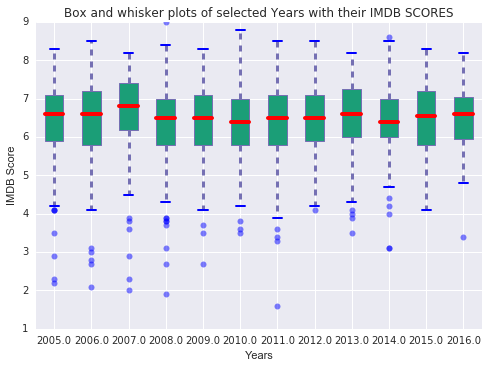
\includegraphics[width=1.0\columnwidth]{Fig/BoxandwhiskerplotofYearsbasedonimdbscore.png}
\caption{IMDB Score based on year}
\label{fig:Box and whisker plotofYearsbasedonimdbscore}
\end{figure}

\begin{figure}
\centering
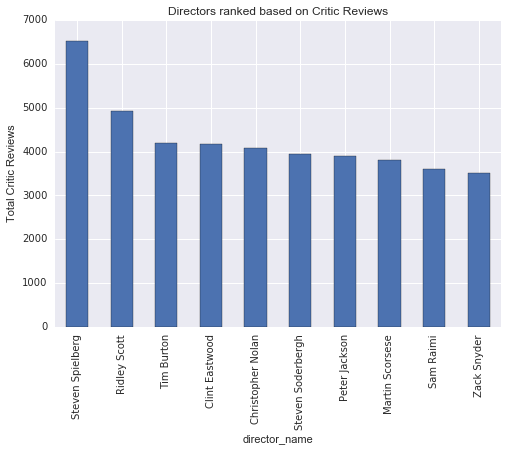
\includegraphics[width=1.0\columnwidth]{Fig/DirectorsRankedontotalcriticreviews.png}
\caption{Top 10 Critics Choice Directors}
\label{fig:Directors Ranked on total critic reviews}
\end{figure}

\begin{figure}
\centering
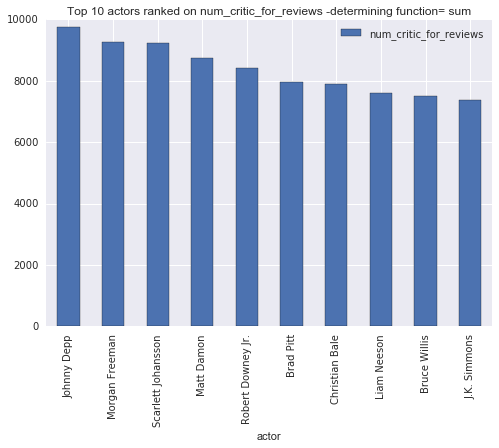
\includegraphics[width=1.0\columnwidth]{Fig/ttanc.png}
\caption{Top 10 Critics Choice Actors}
\label{fig:ttanc}
\end{figure}

\begin{figure}
\centering
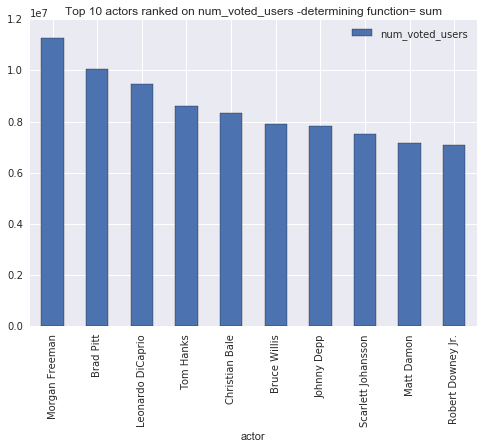
\includegraphics[width=1.0\columnwidth]{Fig/Top10actorsbasedonnumvotedusers.png}
\caption{Top 10 User Voted Actors}
\label{fig:Top10actorsbasedonnumvotedusers}
\end{figure}

\begin{figure}
\centering
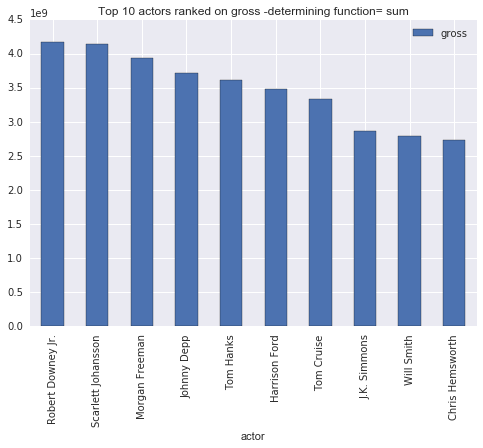
\includegraphics[width=1.0\columnwidth]{Fig/Top10actorsbasedongross.png}
\caption{Top 10 Grossing Actors}
\label{fig:Top10actorsbasedongross}
\end{figure}

\begin{figure}
\centering
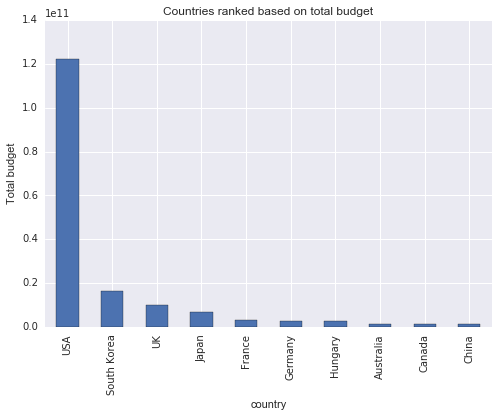
\includegraphics[width=1.0\columnwidth]{Fig/crfm.png}
\caption{Top 10 Countries by Budget}
\label{fig:crfm}
\end{figure}

\begin{figure}
\centering
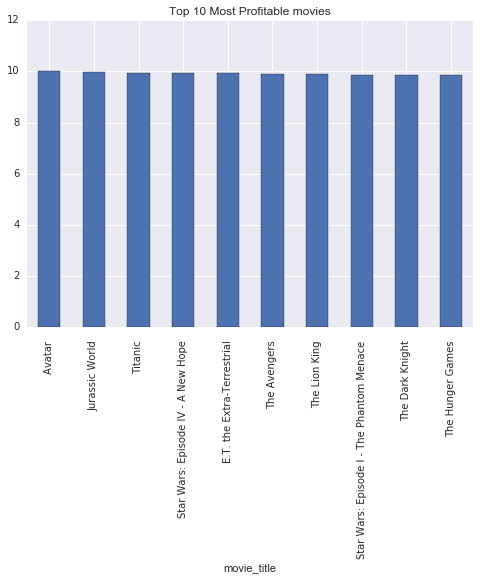
\includegraphics[width=1.0\columnwidth]{Fig/TOP10MostProfitableMovies.png}
\caption{Top 10 Profitable Movies}
\label{fig:TOP10MostProfitableMovies}
\end{figure}

\end{document}
